\section{问题分析}\label{sec:problem_analysis}

三个问题围绕多模态情感识别的不同环节展开，但数据并非逐问传递。问题一使用附件1研究原始视频的三模态特征提取与时序对齐；问题二独立使用附件2研究完整输入和局部连续缺失条件下的情感预测；问题三直接沿用问题二确定的预测模型，进一步分析不同模态及局部输入对预测结果的作用。因此，三问分别解决多模态信息如何表示与对齐、已对齐特征如何用于预测，以及预测结果如何解释。

本文三个问题的输入、处理过程及输出关系如图~\ref{fig:overall_framework}所示。
\begin{figure}[H]
\centering
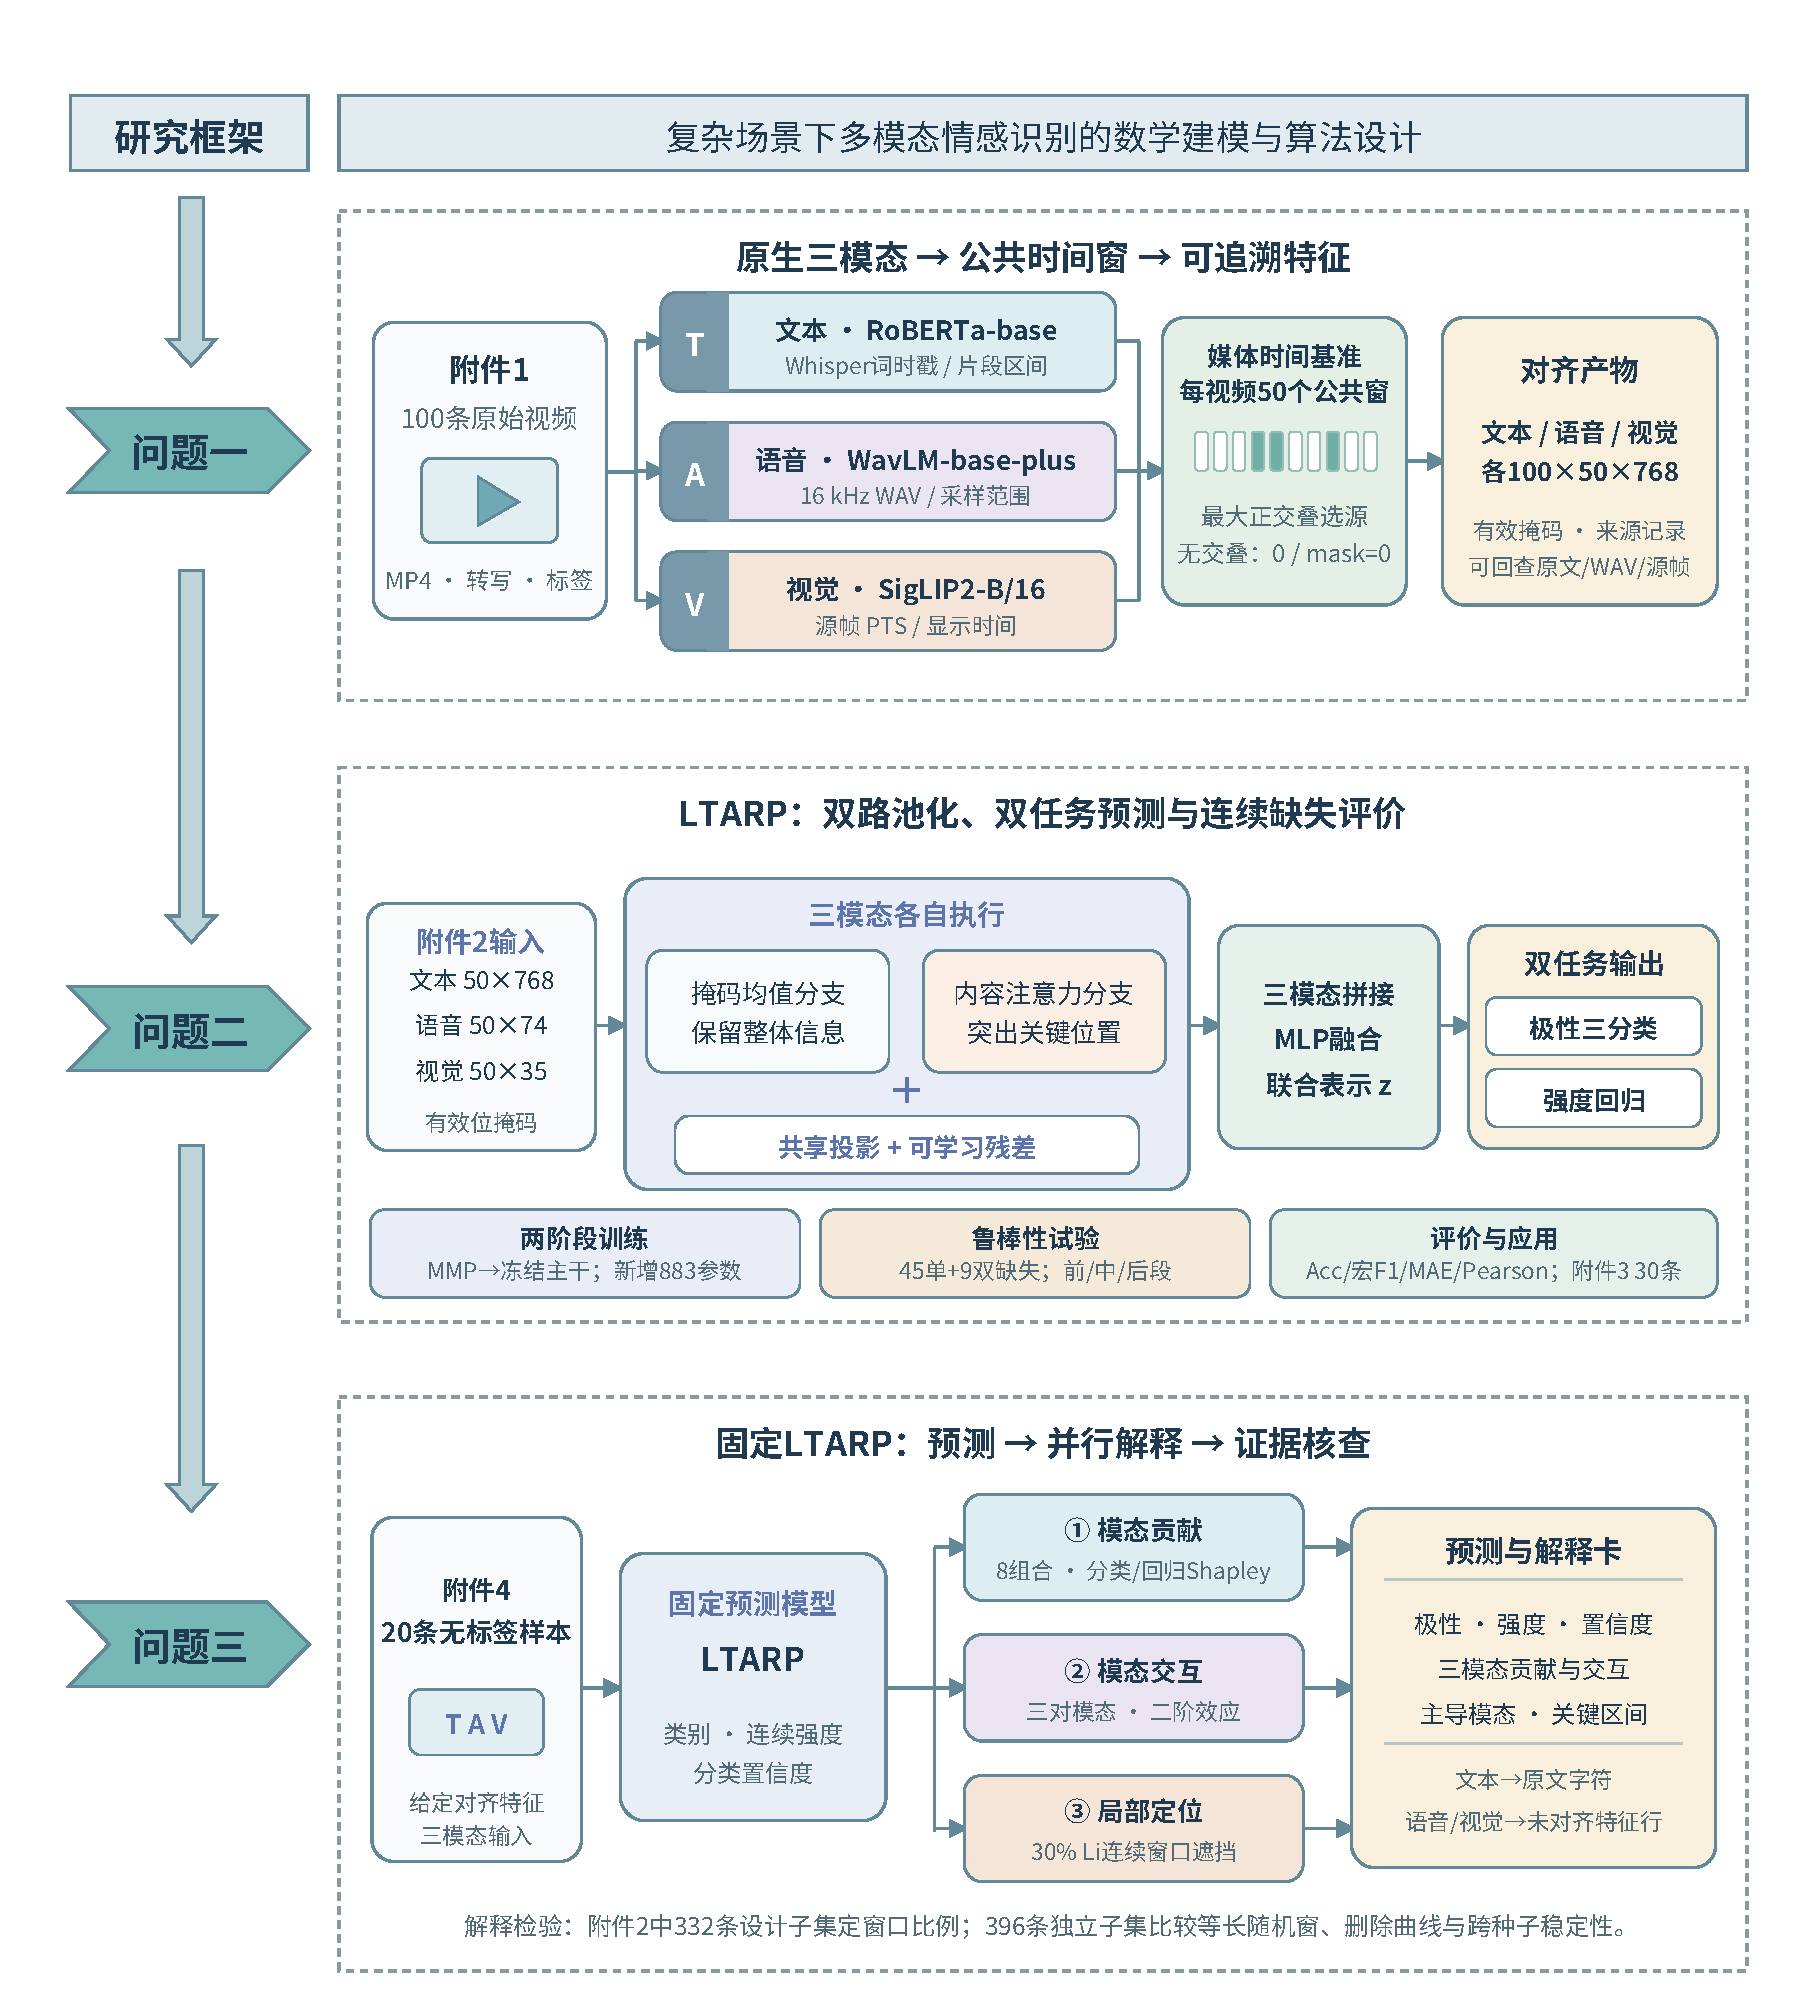
\includegraphics[width=0.94\textwidth]{figures/overall/fig00_overall_framework.pdf}
\caption{全文总体求解框架}
\label{fig:overall_framework}
\end{figure}


问题一的主要困难是三种模态并不共享天然的序列索引。文本对应词语或片段，语音表示更密集，视觉由离散画面构成；采样频率、表示粒度和时间位置均不相同\cite{bagherzadeh2018mosei}。直接对相同索引拼接，可能把不同媒体时刻的内容并置。需要先提取各自特征和时间位置，再用共同的媒体时间表示组织它们，同时保留可回查的来源。

问题二使用已给出的对齐特征，重点转为不同观测条件下的预测。局部连续缺失不仅减少可用内容，还改变剩余信息在序列中的分布；相同缺失长度发生在不同模态或位置，结果也可能不同。因而需要以基础聚合方式建立可比较的参照，再考虑剩余位置的信息差异。评价须同时涵盖分类与回归、完整输入与连续缺失输入，才能区分总体表现和受损后的保持程度。

问题三面对的是预测结果的可理解性。类别或强度本身不能说明哪一路输入发挥作用，也不能说明模态联合输入是否改变作用方式，更不能指出影响来自序列中的哪一段。解释应从单个模态推进到模态组合，再细化到局部位置；局部索引还需联系实际输入记录，明确可追溯的范围。

其中，附件1用于特征构建与来源回查，附件2用于预测模型的训练与评价，附件3和附件4分别用于无标签预测及预测解释。

基于上述分析，后文先说明共用的建模前提与核心符号，再依次给出三个问题的模型、实验与结果。

